\documentclass[oneside,a4paper,14pt]{extarticle}
\usepackage[a4paper,top=20mm,bottom=20mm,left=30mm,right=10mm]{geometry}
\usepackage{amsmath, amssymb, amsfonts, amsthm}
\usepackage[T2A]{fontenc}
\usepackage[utf8]{inputenc}
\usepackage[russian]{babel}
\usepackage{textcomp}
\usepackage{indentfirst}
\usepackage{graphicx}
\usepackage{float}
\usepackage{wrapfig}
\usepackage{caption}
\usepackage{amsmath}
\usepackage{tocloft}
\usepackage{multicol}
\renewcommand{\cftsecleader}{\cftdotfill{\cftdotsep}}
\usepackage[breaklinks]{hyperref}
\usepackage{titlesec}
\usepackage{fancyvrb}
\usepackage{xcolor}
\newcommand{\xr}[1]{\xrightarrow{\text{#1}}}
\titleformat{\section}{\normalsize\bfseries}{\thesection}{1em}{}
\titleformat{\subsection}{\normalsize\bfseries}{\thesubsection}{1em}{}
\titleformat{\subsubsection}{\normalsize\bfseries}{\thesubsubsection}{1em}{}
\renewcommand\baselinestretch{1.33}\normalsize
\setlength{\parindent}{1.25cm}

\begin{document}




\section*{Цель}
\addcontentsline{toc}{section}{Цель}
Изучить базовые принципы построения формальной грамматики, выполнив задание на создание правил вывода для порождения имён из заданного алфавита.


\section*{Терминальыне символы}
\addcontentsline{toc}{section}{Терминальыне символы}
$V_T = \{ \text{и}, \text{в}, \text{а}, \text{н},\text{л},\text{д},\text{м} \}$


\section*{Нетерминальыне символы}
\addcontentsline{toc}{section}{Нетерминальыне символы}
$V_T = \{ \text{С}, \text{А}, \text{Б}\}$


\section*{Правила}
\addcontentsline{toc}{section}{Правила}
\begin{multicols}{2}
\begin{enumerate}
    \item $ \text{С} \to \text{в}\text{А}$
    \item $ \text{С} \to \text{д}\text{А}$
    \item $ \text{С} \to \text{м}\text{Б}$
    \item $ \text{С} \to \text{а}\text{Б}$
    \item $ \text{С} \to \text{А}$
    \item $ \text{А} \to \text{и}\text{Б}$
    \item $ \text{А} \to \text{л}\text{С}$
    \item $ \text{А} \to \epsilon$
    \item $ \text{А} \to \text{С}$
    \item $ \text{Б} \to \text{н}\text{А}$
    \item $ \text{Б} \to \text{А}$
    \item $ \text{Б} \to \text{С}$
\end{enumerate}
\end{multicols}

\section*{Цепочки}
\addcontentsline{toc}{section}{Цепочки}
\begin{enumerate}
    \item$
    \text{С}        \xr{4}
    \text{аБ}       \xr{11}
    \text{аА}       \xr{7}
    \text{алС}      \xr{5}
    \text{алА}      \xr{6}
    \text{алиБ}     \xr{10}
    \text{алинА}    \xr{9}
    \text{алинС}    \xr{4}
    \text{алинаБ}   \xr{11}
    \text{алинаА}   \xr{8}
    \text{алина}
    $
    \item$
    \text{С}        \xr{3}
    \text{мБ}       \xr{11}
    \text{мА}       \xr{6}
    \text{миБ}      \xr{11}
    \text{миА}      \xr{7}
    \text{милС}     \xr{4}
    \text{милаБ}    \xr{10}
    \text{миланА}   \xr{9}
    \text{миланС}   \xr{4}
    \text{миланаБ}  \xr{11}
    \text{миланаА}  \xr{8}
    \text{милана}
    $
    \item$
    \text{С}        \xr{2}
    \text{дА}       \xr{6}
    \text{диБ}      \xr{12}
    \text{диС}      \xr{4}
    \text{диаБ}     \xr{10}
    \text{дианА}    \xr{9}
    \text{дианС}    \xr{4}
    \text{дианаБ}   \xr{11}
    \text{дианаА}   \xr{8}
    \text{диана}
    $
    \item$
    \text{С}        \xr{2}
    \text{дА}       \xr{9}
    \text{дС}       \xr{4}
    \text{даБ}      \xr{10}
    \text{данА}     \xr{6}
    \text{даниБ}    \xr{11}
    \text{даниА}    \xr{6}
    \text{данииБ}   \xr{11}
    \text{данииА}   \xr{7}
    \text{даниилС}  \xr{5}
    \text{даниилА}  \xr{8}
    \text{даниил}
    $
    \item$
    \text{С}        \xr{1}
    \text{вА}       \xr{7}
    \text{влС}      \xr{4}
    \text{влаБ}     \xr{12}
    \text{влаС}     \xr{2}
    \text{владА}    \xr{9}
    \text{владС}    \xr{4}
    \text{ввладаБ}  \xr{11}
    \text{владаА}   \xr{8}
    \text{влада}
    $
    \item$
    \text{С}        \xr{1}
    \text{вА}       \xr{9}
    \text{вС}       \xr{4}
    \text{ваБ}      \xr{12}
    \text{ваС}      \xr{2}
    \text{вадА}     \xr{6}
    \text{вадиБ}    \xr{12}
    \text{вадиС}    \xr{3}
    \text{вадимБ}   \xr{11}
    \text{вадимА}   \xr{8}
    \text{вадим}
    $
\end{enumerate}


\section*{Лабораторная в программе}
\addcontentsline{toc}{section}{Лабораторная в программе}
\begin{figure}[H]
    \centering
    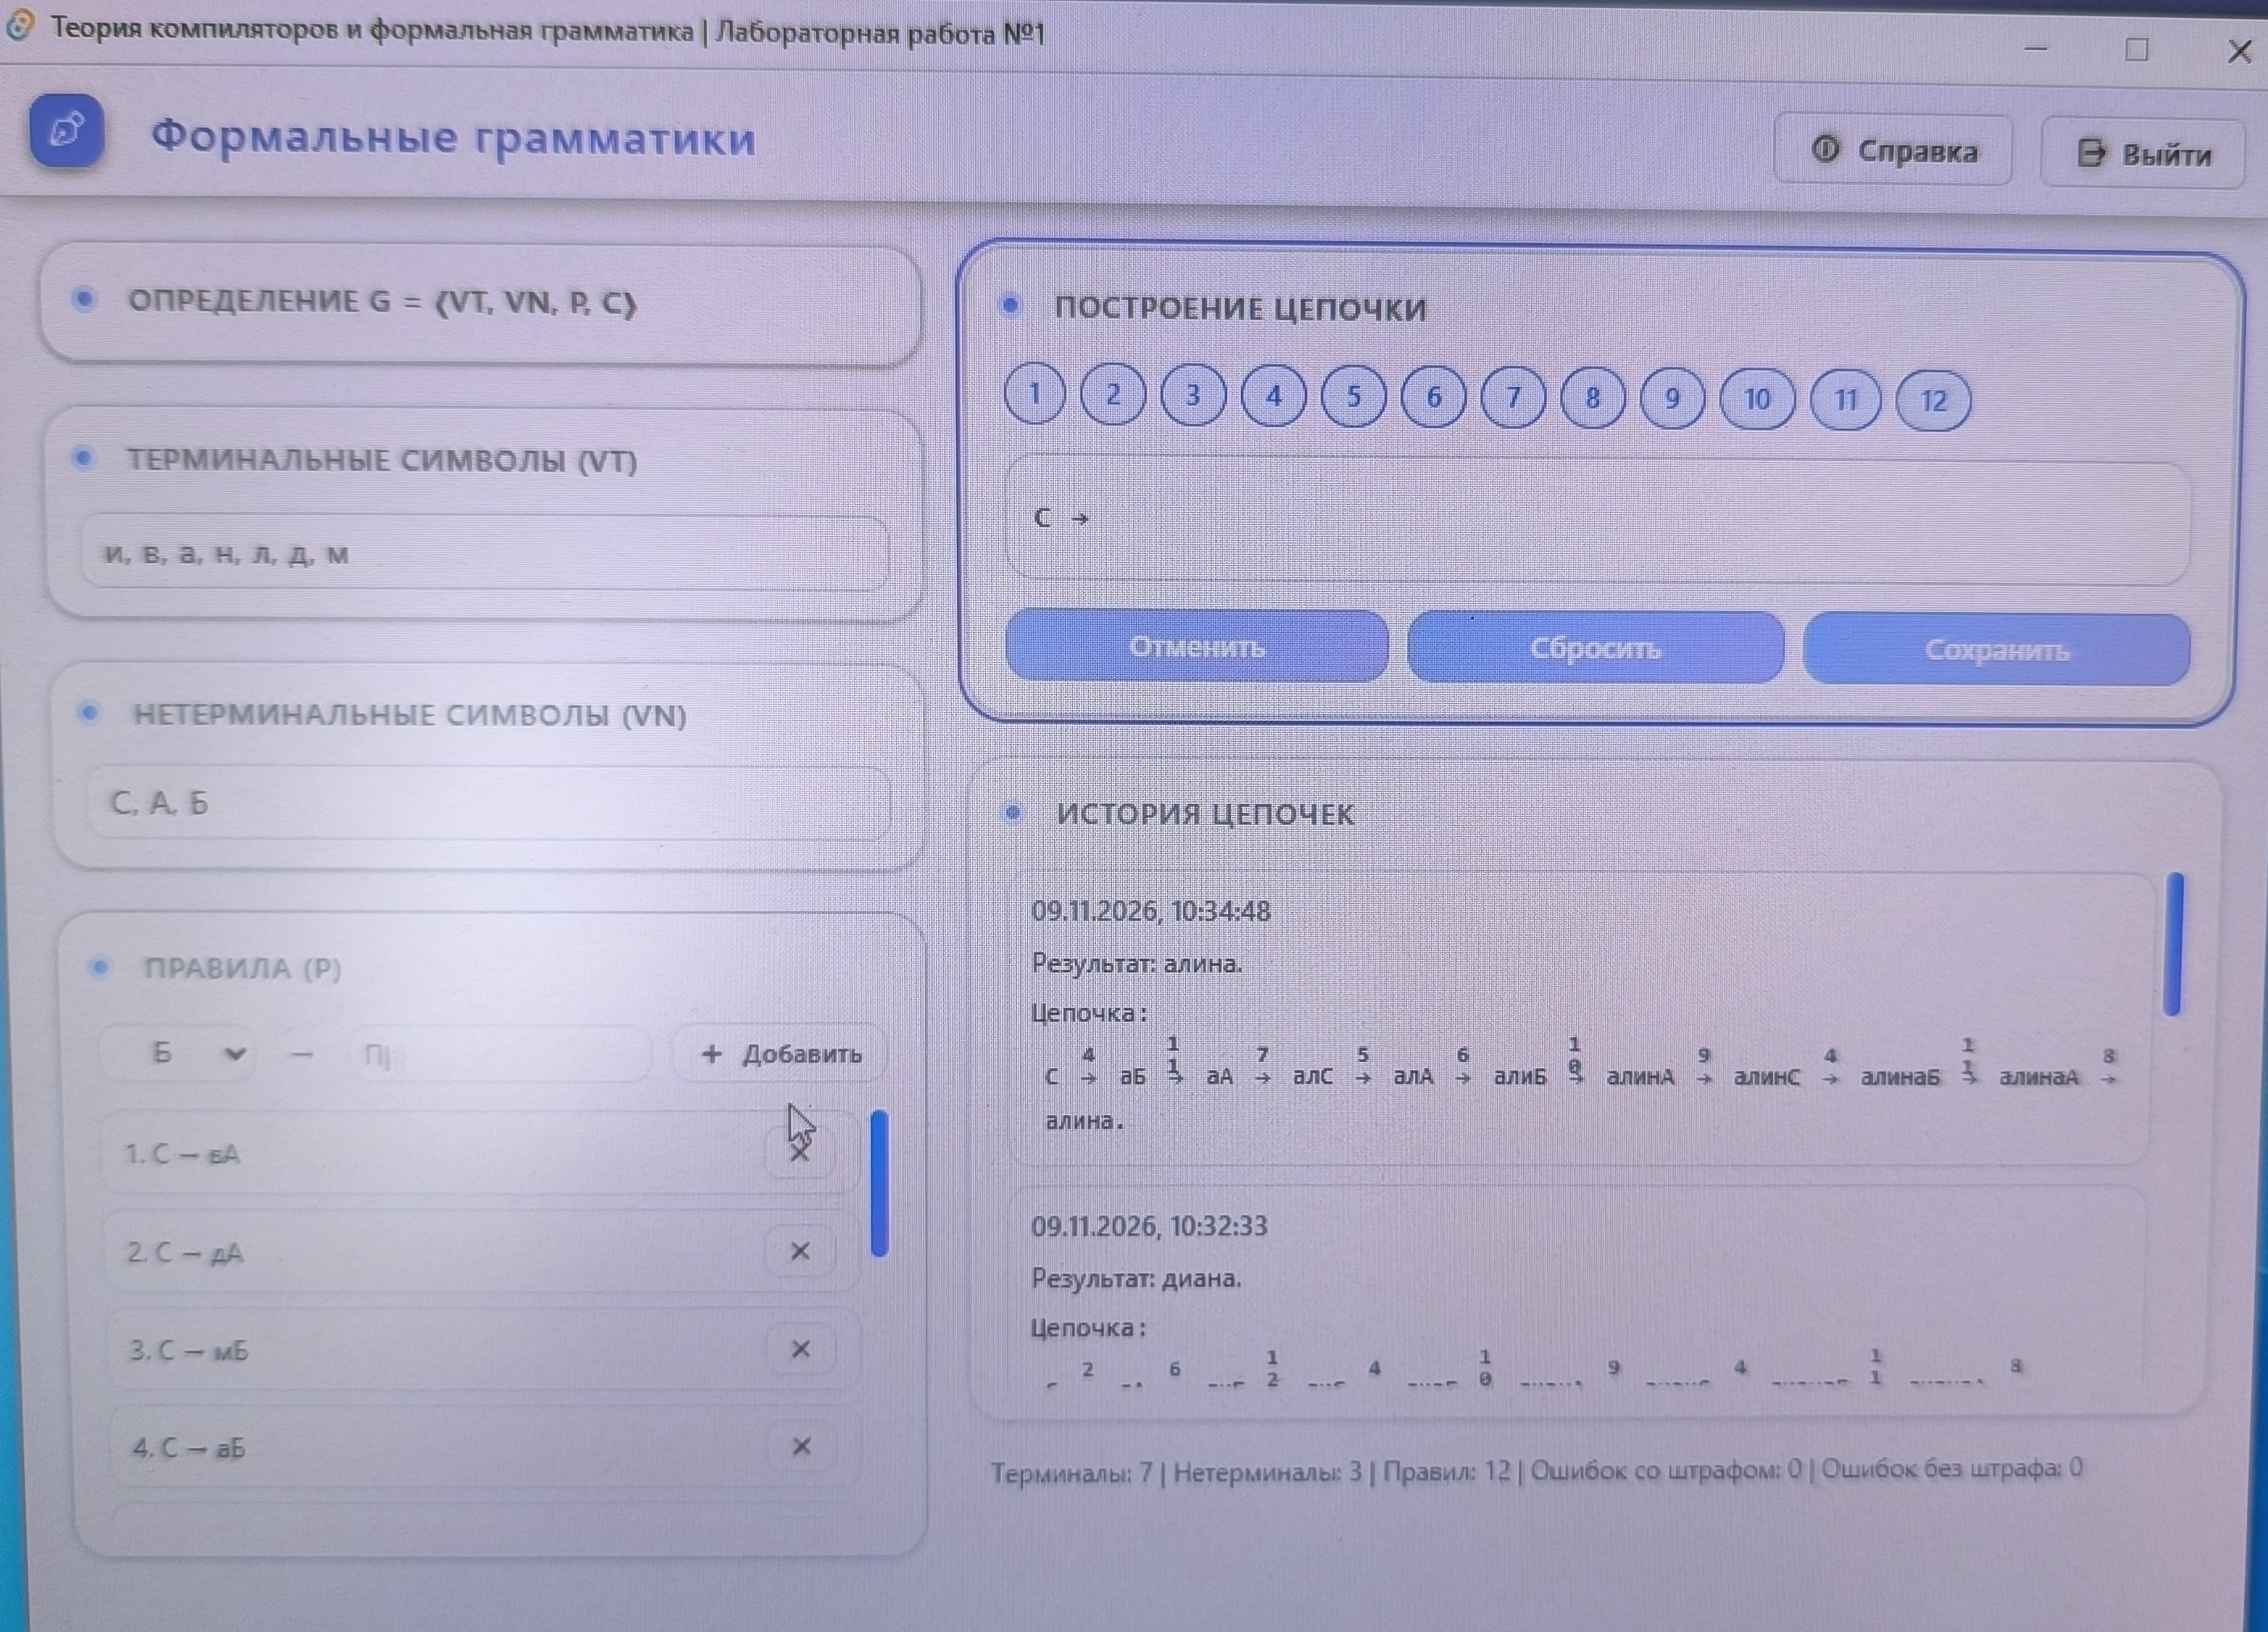
\includegraphics[width=0.8\textwidth]{лаба1 (1).jpg}
    \caption{Первые правила и цепочки}
    \label{fig:scr1}
\end{figure}
\begin{figure}[H]
    \centering
    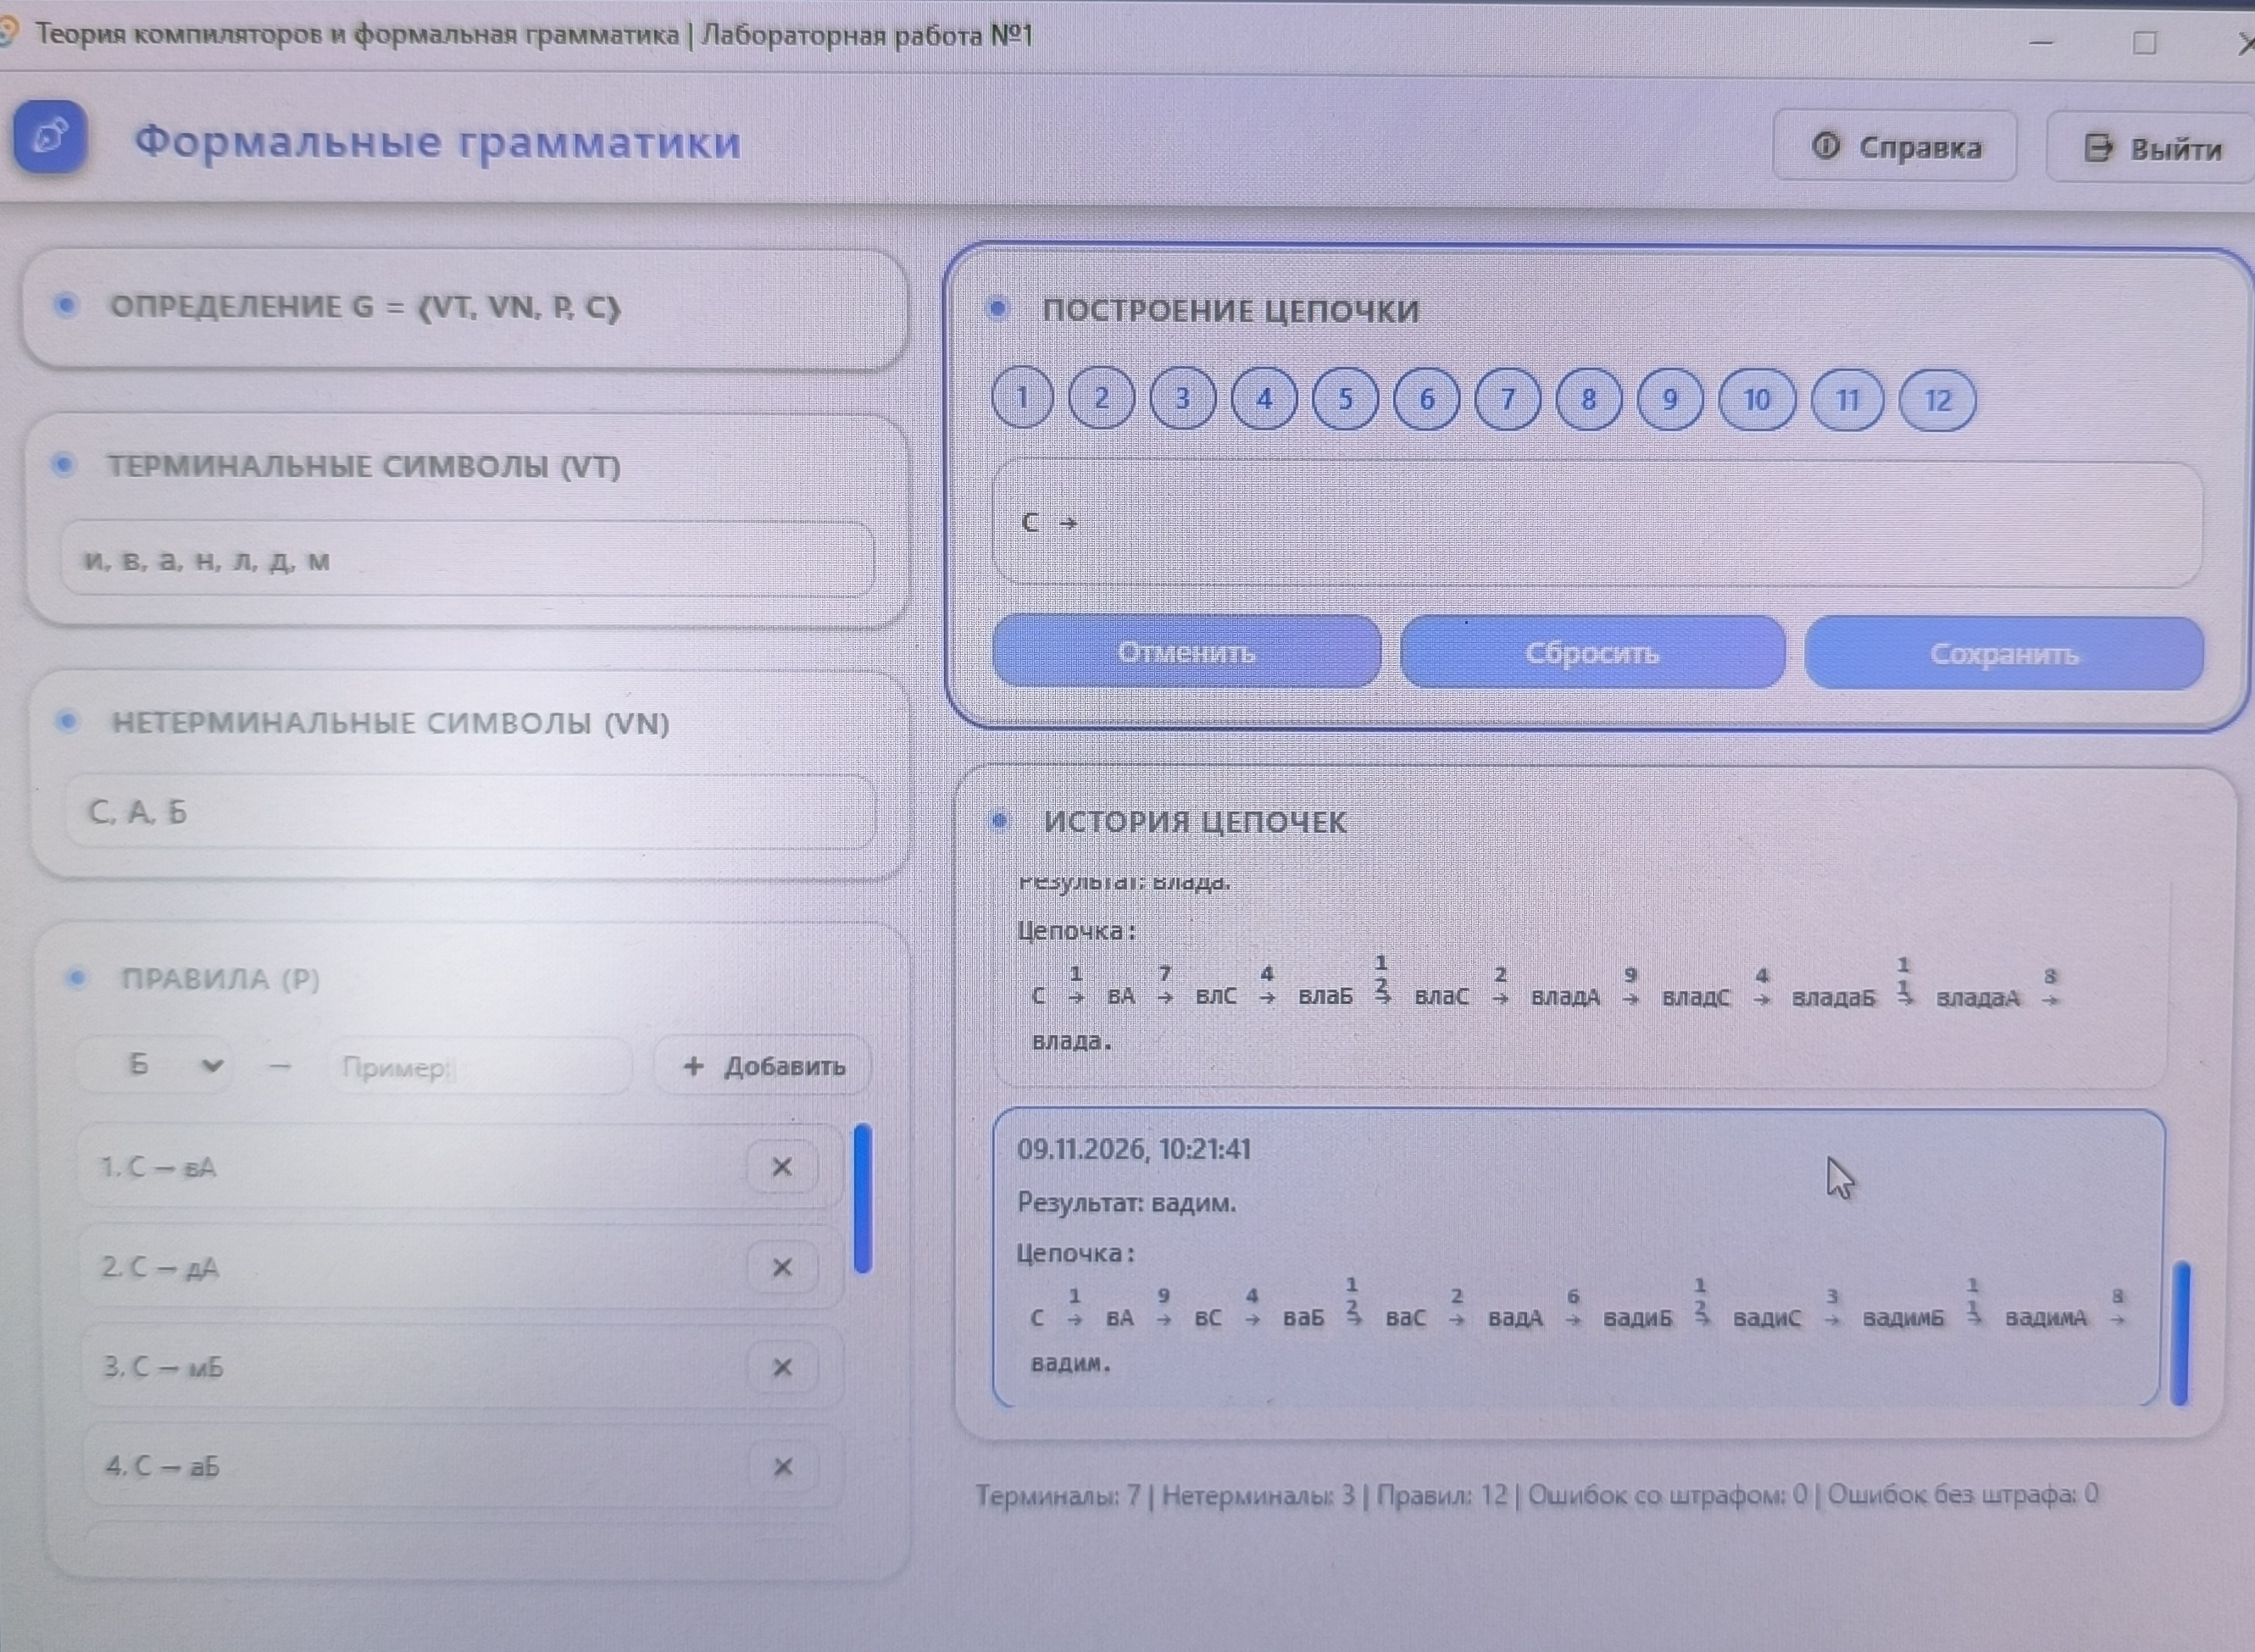
\includegraphics[width=0.8\textwidth]{лаба1 (2).jpg}
    \caption{Последние правила и цепочки}
    \label{fig:scr2}
\end{figure}


\section*{Вывод}
\addcontentsline{toc}{section}{Вывод}
В ходе выполнения лабораторной работы были сделаны правила формальной грамматики, позволяющие
породить имена длиной от пяти символов, используя заданного алфавита.



\end{document}